\documentclass[12pt,a4paper,notitlepage]{article}
\usepackage[utf8]{inputenc}
\usepackage[english]{babel}
\usepackage[T1]{fontenc}
\usepackage[backend=biber,
			style=authoryear-comp,
			isbn=false,
			doi=false,
			bibstyle=authoryear,
			natbib,
			]{biblatex}
\usepackage{eurosym}
\usepackage{enumitem}
\usepackage{url}
\usepackage{blindtext}
\usepackage{hyperref}
\usepackage{breakurl}
\usepackage{amsmath}
\usepackage{titling}
\usepackage{amsfonts}
\usepackage{amssymb}
\usepackage{pgfplots}
\usepackage{caption}
\usepackage{subcaption}
\usepackage{graphicx}
\usepackage{dcolumn}
\usepackage{tikz-3dplot}
\usepackage{subcaption}
\usepackage{float}
\usepackage{adjustbox}
\usepackage{multirow,rotating}
\usepackage[autostyle]{csquotes}
\usepackage[toc,page]{appendix}
\usepackage{lscape}
\usepackage{todonotes}
\usepackage{booktabs}
\usepackage{multirow}
\usepackage{bm}
\usepackage{eurosym}

\begin{document}

\section{Introduction}

Social networks such as Facebook are becoming more and more important for online news services: an increasing number of their readers access the news pages via links in the networks. Users of Facebook, for example, can use their profile to share links to external websites - such as news portals - with their online friends. This has led to the development of social media into an important generator of traffic on the internet pages. In Germany, 94\% of online shared news articles in 2015 are distributed via Facebook, followed by Twitter with 3.5\% and Google+ with 2.3\% \citep{schiller_development_2016}. The advertising-financed business model of the media houses is based on the premise that users visit their websites in order to achieve high advertising revenues. For this reason, news agencies are particularly interested in finding out which topics are more likely shared on these platforms. \citet{schiller_development_2016} show, that social media users choose a certain site depending on the researched topic. FOCUS Online for example is targeted for articles from politics and business, sports news is more likely to be shared from Bild.de. 

While these static resorts give an indication on the content of an article, multiple articles in the same resort probably don't cover the same topics (and are not equally shared). Especially if the articles originate from different news portals. Furthermore, articles can contain more than one topic. We use a structural topic model to reveal the underlying topics of a collection of articles (a corpus), and how the articles exhibit them. We then estimate the effect of topic prevalence on the number of Facebook shares. 

Mapping raw text to one or more topics, without having prior knowledge on what those topics are, translates to an unsupervised classification problem on natural language. Within topic models the Latent Dirichlet Allocation (LDA) is a widely used technique, where each document (article) is viewed as a mixture of topics (represented by the document-topic distribution) and each topic is a mixture of unique terms (represented by the topic-term distribution).\cite{blei_latent_2003} 

LDA makes a statistical assumption that all texts in the modeled corpus are generated by the same underlying process \citep{blei_latent_2003}. Thus, it is not ideally suited to examining differences in topical content that are affected by covariates such as author identity or time of writing. \citet{roberts_model_2016} develop a structural topic model (STM) that allows to incorporate external variables that effect both topical content and topical prevalence. We use this approach to analyze online news about the german federal elections, where we allow prevalence of topics to vary across newswire services. We then estimate the effect of topical prevalence (the posterior document-topic distribution) on the number of Facebook shares.

Figure \ref{fig_research_strat} gives an overview of the applied research strategy. Chapter \ref{ch_data} contains a description of the text data and how it was pre-processed in order to use it as input variable. Chapter \ref{ch_model} explains the generative process of the mixed membership model and the results of this process are presented in chapter \ref{ch_results}. Chapter \ref{ch_regression} describes how we regress the estimated probabilities of topic prevalence of a document on the times, this document was shared on Facebook.

\begin{figure}[ht]
	\centering
	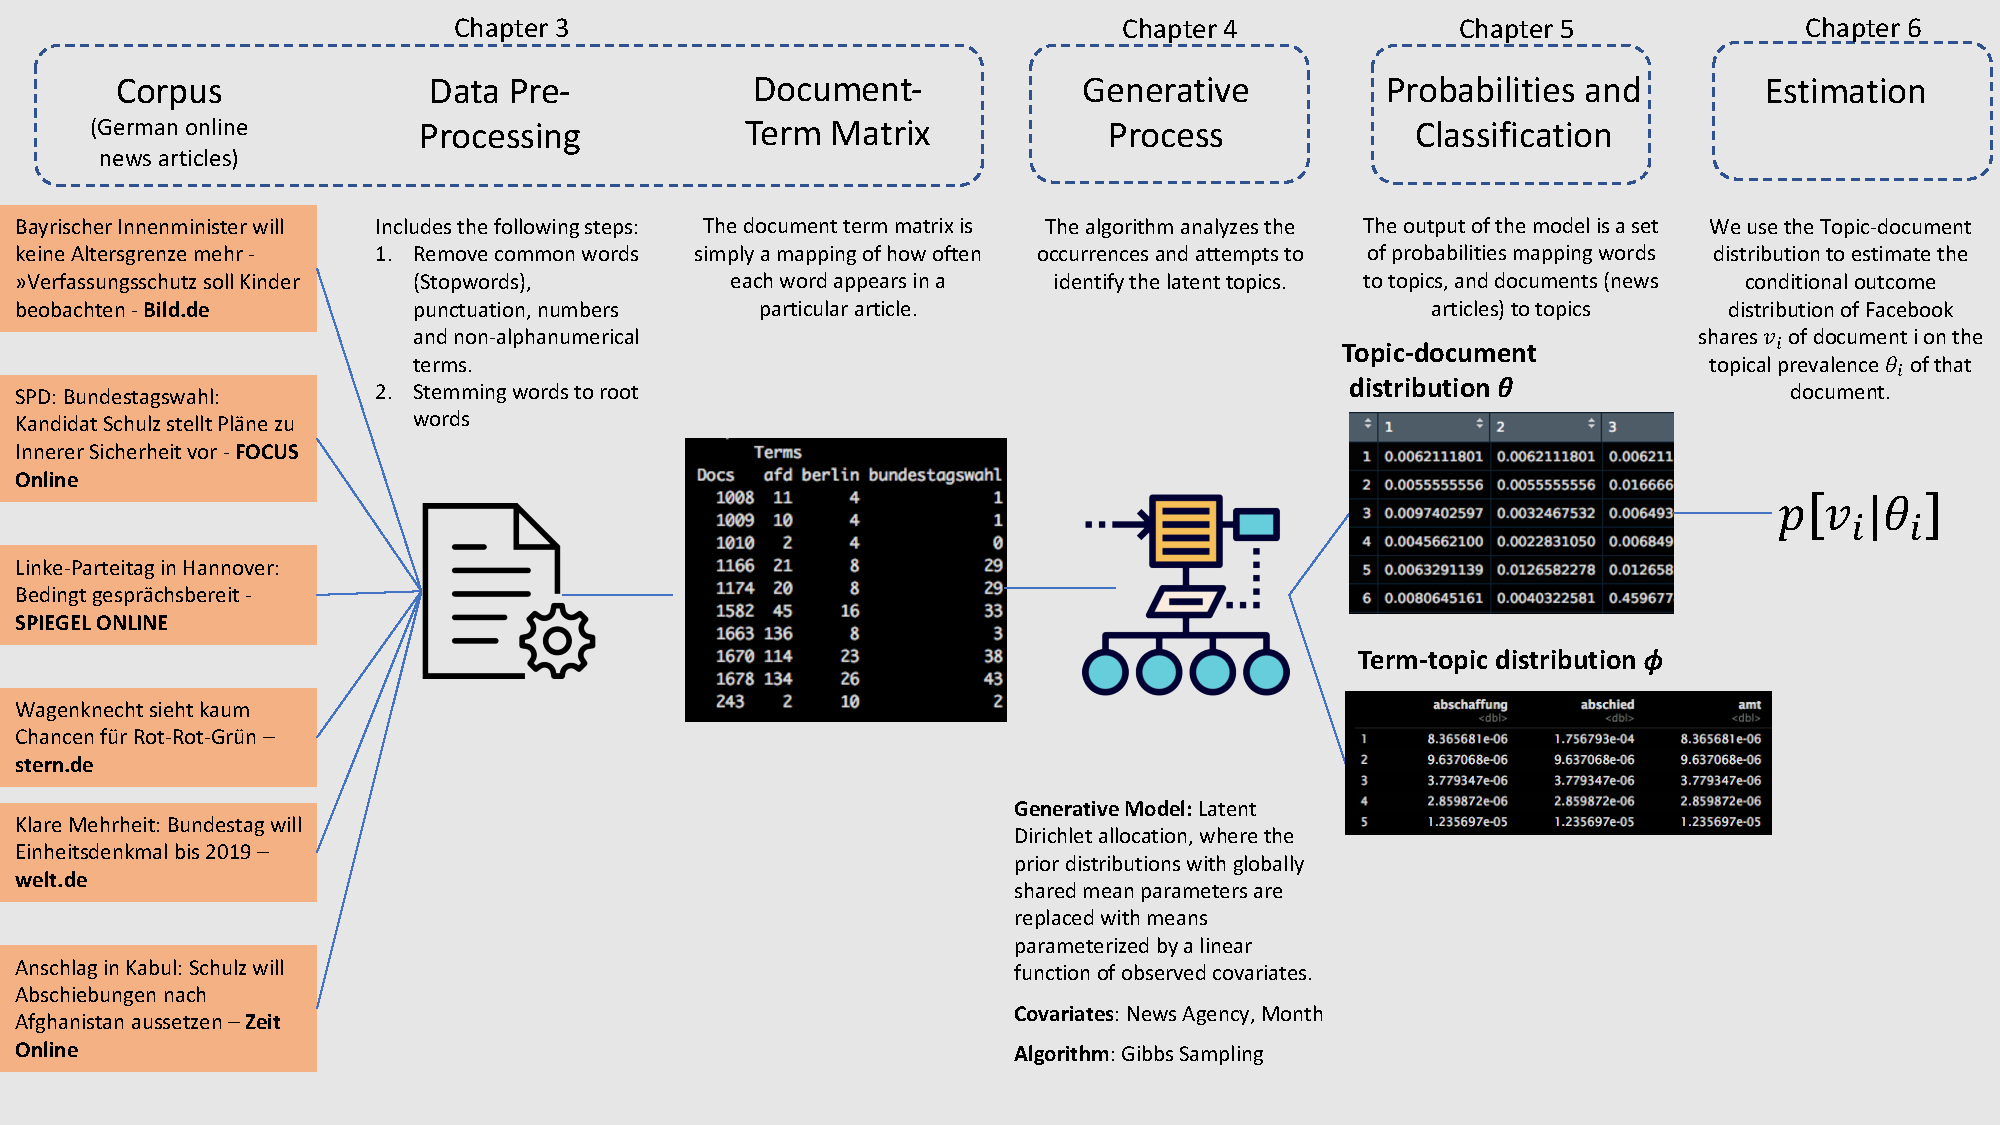
\includegraphics[width=0.95\textwidth]{../figs/research_strategy.pdf} 
	\caption{Research Strategy}
	\label{fig_research_strat}
\end{figure}

% Related Literature
% ------------------

\section{Related Literature}

% Quantitative approaches
% -----------------------


% Topic Modeling / LDA
% ---------------------------

Topic modeling is a statistical and computational technique for discerning information about the contents of a large corpus of documents without reading or annotating the original texts. A topic model uncovers patterns of word co-occurrence across the corpus, yielding a set of word clusters, together with associated probabilities of occurrence, which constitute the topics.

See \citep{taddy_estimation_2012} for a review of topic estimation techniques)

Since its introduction into text analysis, topic modeling has become hugely popular.8 (See \citet{blei_probabilistic_2012} for an overview.) The model has been especially useful in political science (e.g., \citep{grimmer_bayesian_2010}), where researchers have been successful in attaching political issues and beliefs to the estimated latent topics.

Topic modeling is alternatively labeled as “latent Dirichlet allocation,” (LDA) which refers to the Bayesian model in \citet{blei_latent_2003} that treats each $\boldsymbol{v}_i$ and $\boldsymbol{\theta}_l$ as generated from a Dirichlet - distributed prior.
The same model was independently introduced in genetics by \citet{pritchard_inference_2000} for factorizing gene expression as a function of latent populations; it has been similarly successful in that field. 

The basic topic model has been generalized and extended in variety of ways. A prominent example is the dynamic topic model of \citet{blei_dynamic_2006}, which considers documents that are indexed by date (e.g., publication date for academic articles) and allows the topics, say $\boldsymbol{\Theta}_t$, to evolve smoothly in time. 

% Structural topic models (STM)
% ----------------------------
A typical application of topic modeling in the social sciences first estimates LDA, then uses estimates of $\theta_d$ as the dependent variable in an regression on covariates to test whether different types of documents have different content. 

This is contradictory because documents are assumed to be generated by a statistical process that we subsequently reject.

The structural topic model (STM) of Roberts et. al. (2016) explicitly introduces covariates into a topic model, and allows one to estimate the impact of document-level covariates on topic content and prevalence as part of the topic model itself.

% -----
% Data
% -----

\section{Dataset}\label{ch_data}

We conduct our estimation on a sample of 10531 news articles containing the term "Bundestagswahl" (Federal Election) dated from 01.06.2017 to 28.10.2017.\footnote{German federal elections took place on 24th of September 2017.} We first extract all online articles of six mainstream german online news portals\footnote{Bild.de, Focus.de, Spiegel.de, Stern.de, Welt.de, Zeit.de} using the the Event Regestry API.\footnote{For more information see http://eventregistry.org/documentation. The scraping code was written in Python and can be made available on request.} We then filter those articles that contain the term "Bundestagswahl" (Federal Election) in their text body. 

Figure \ref{fig_distr} shows the distribution of the number of articles from the respective news sources by date. There is a high peak around the federal elections on September, 24th. Most of the articles are published by welt.de, followed by stern.de.  

\begin{figure}[H]
	\caption{Article distribution...}
	\begin{center}
		\begin{subfigure}[normla]{0.49\textwidth}
			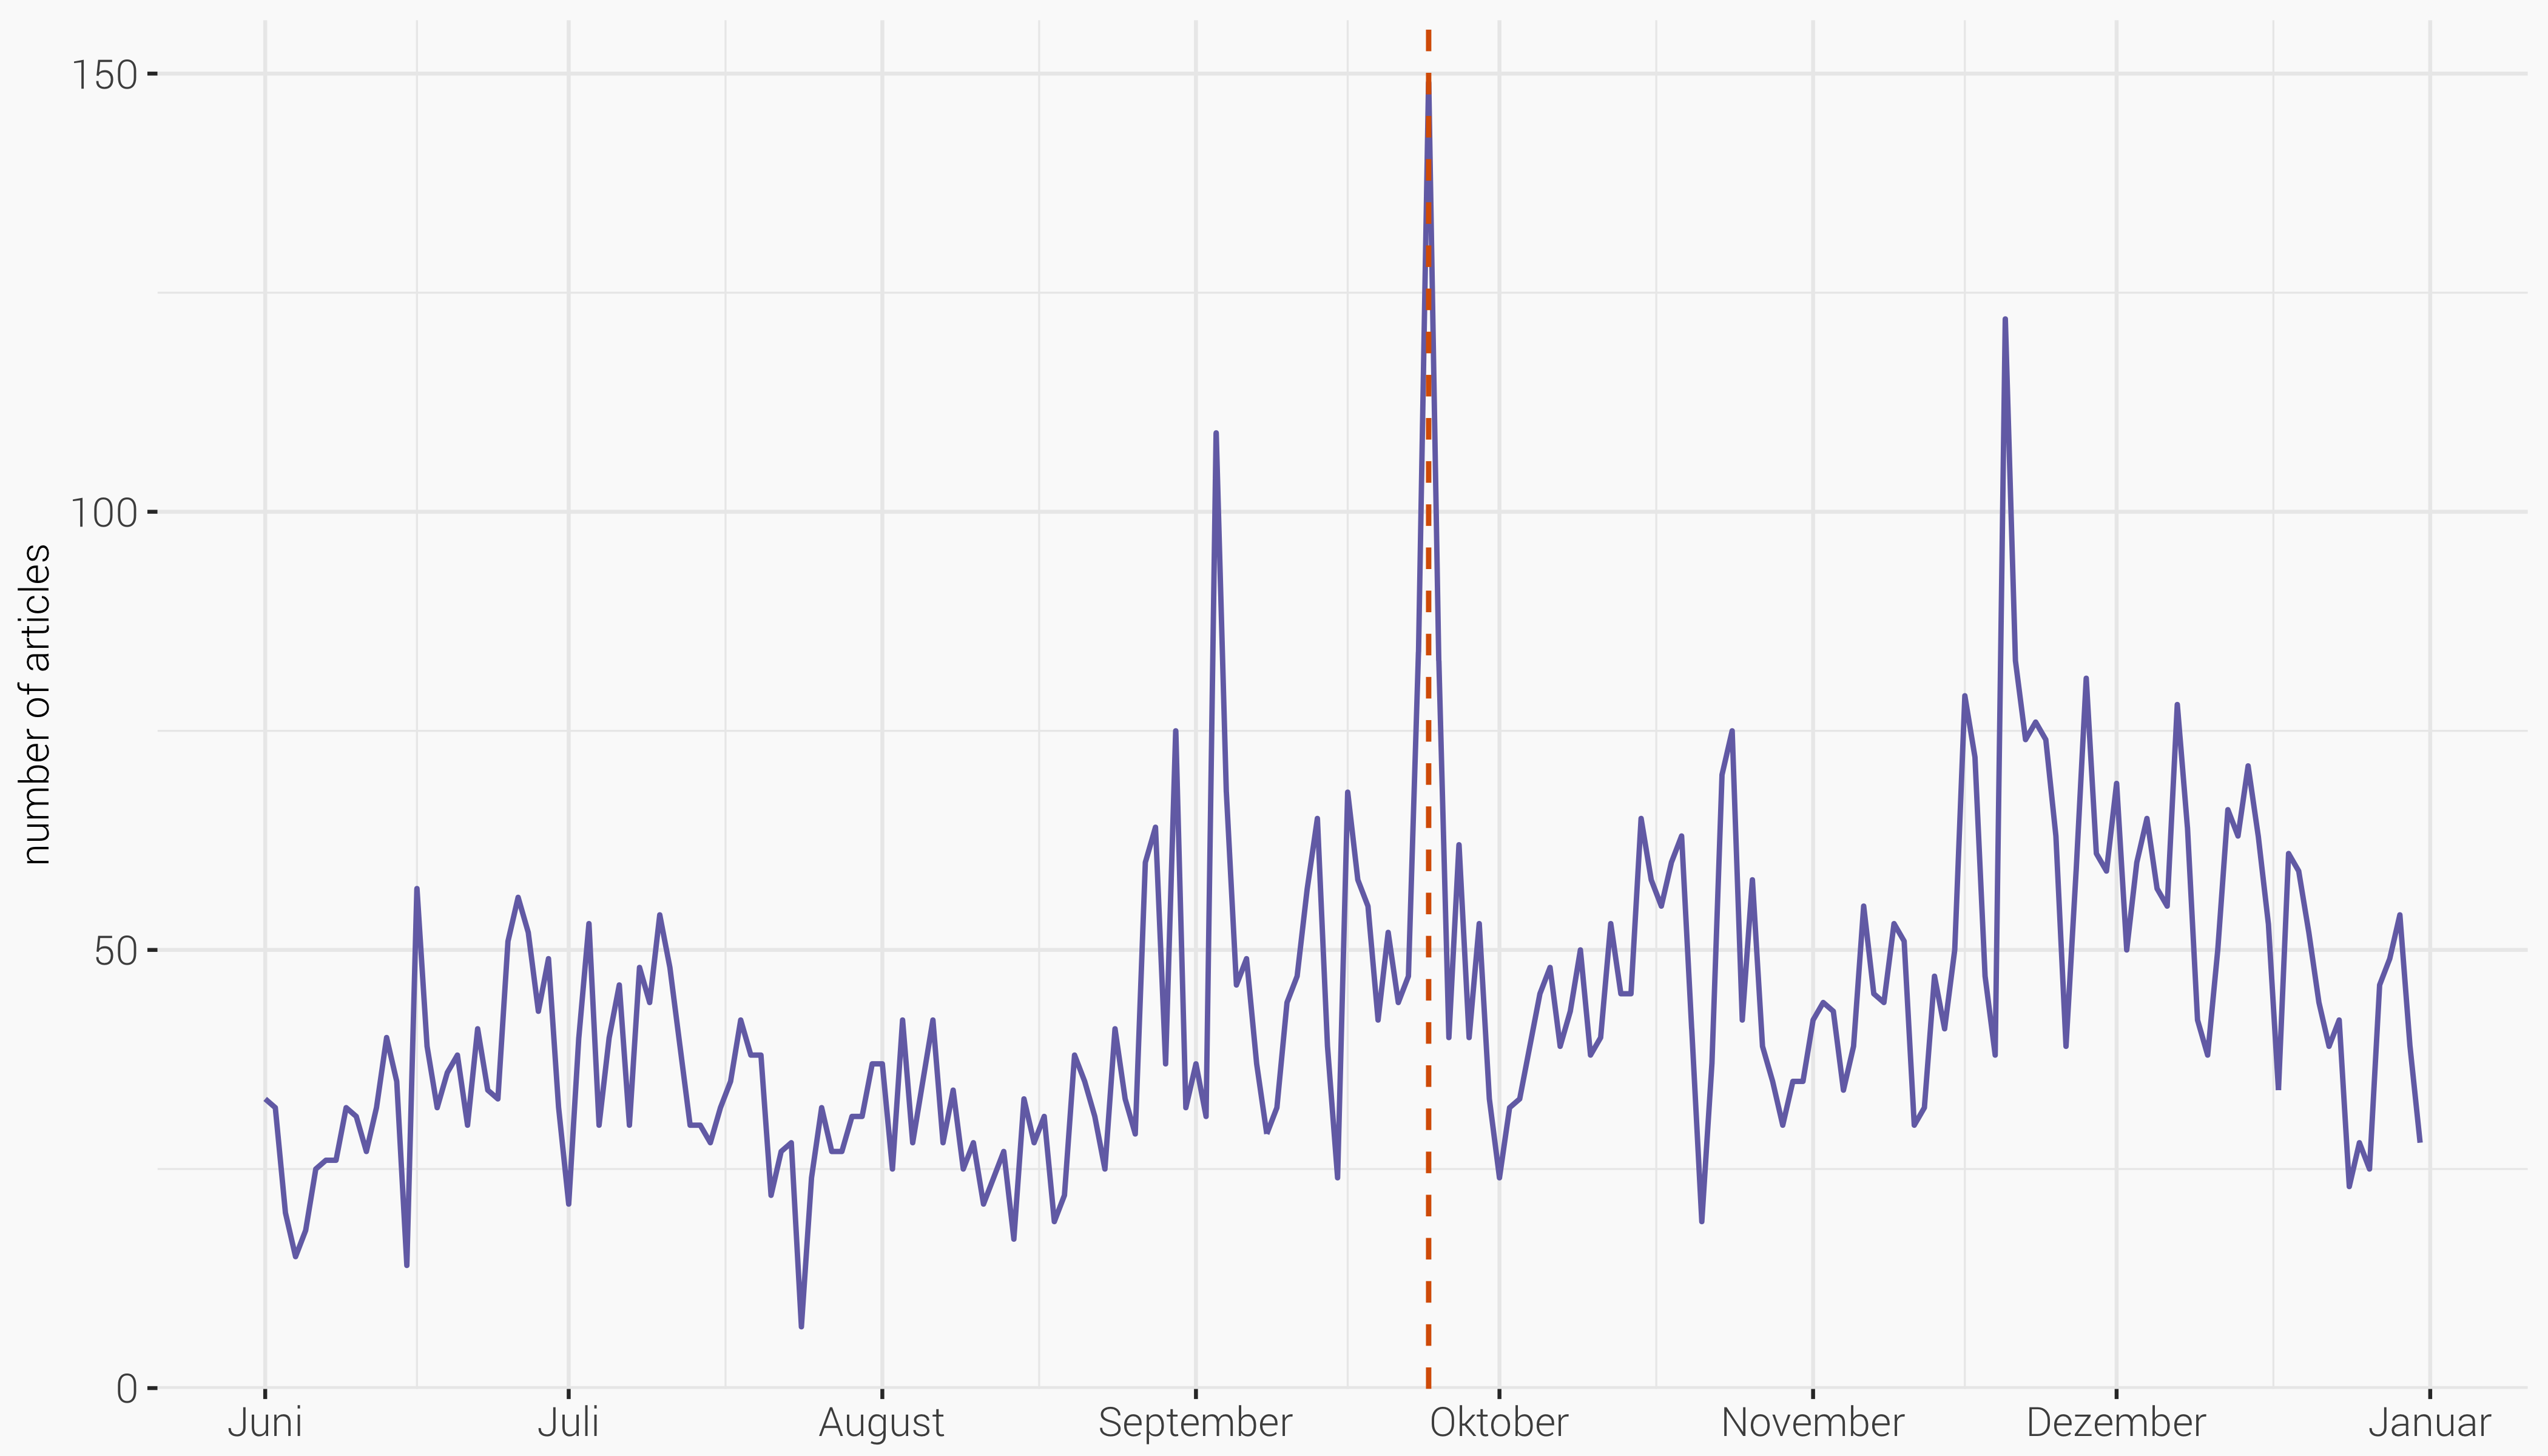
\includegraphics[width=\textwidth]{../figs/timeline.png}
			\caption{...by date \& news source}
		\end{subfigure}
		\begin{subfigure}[normla]{0.49\textwidth}
			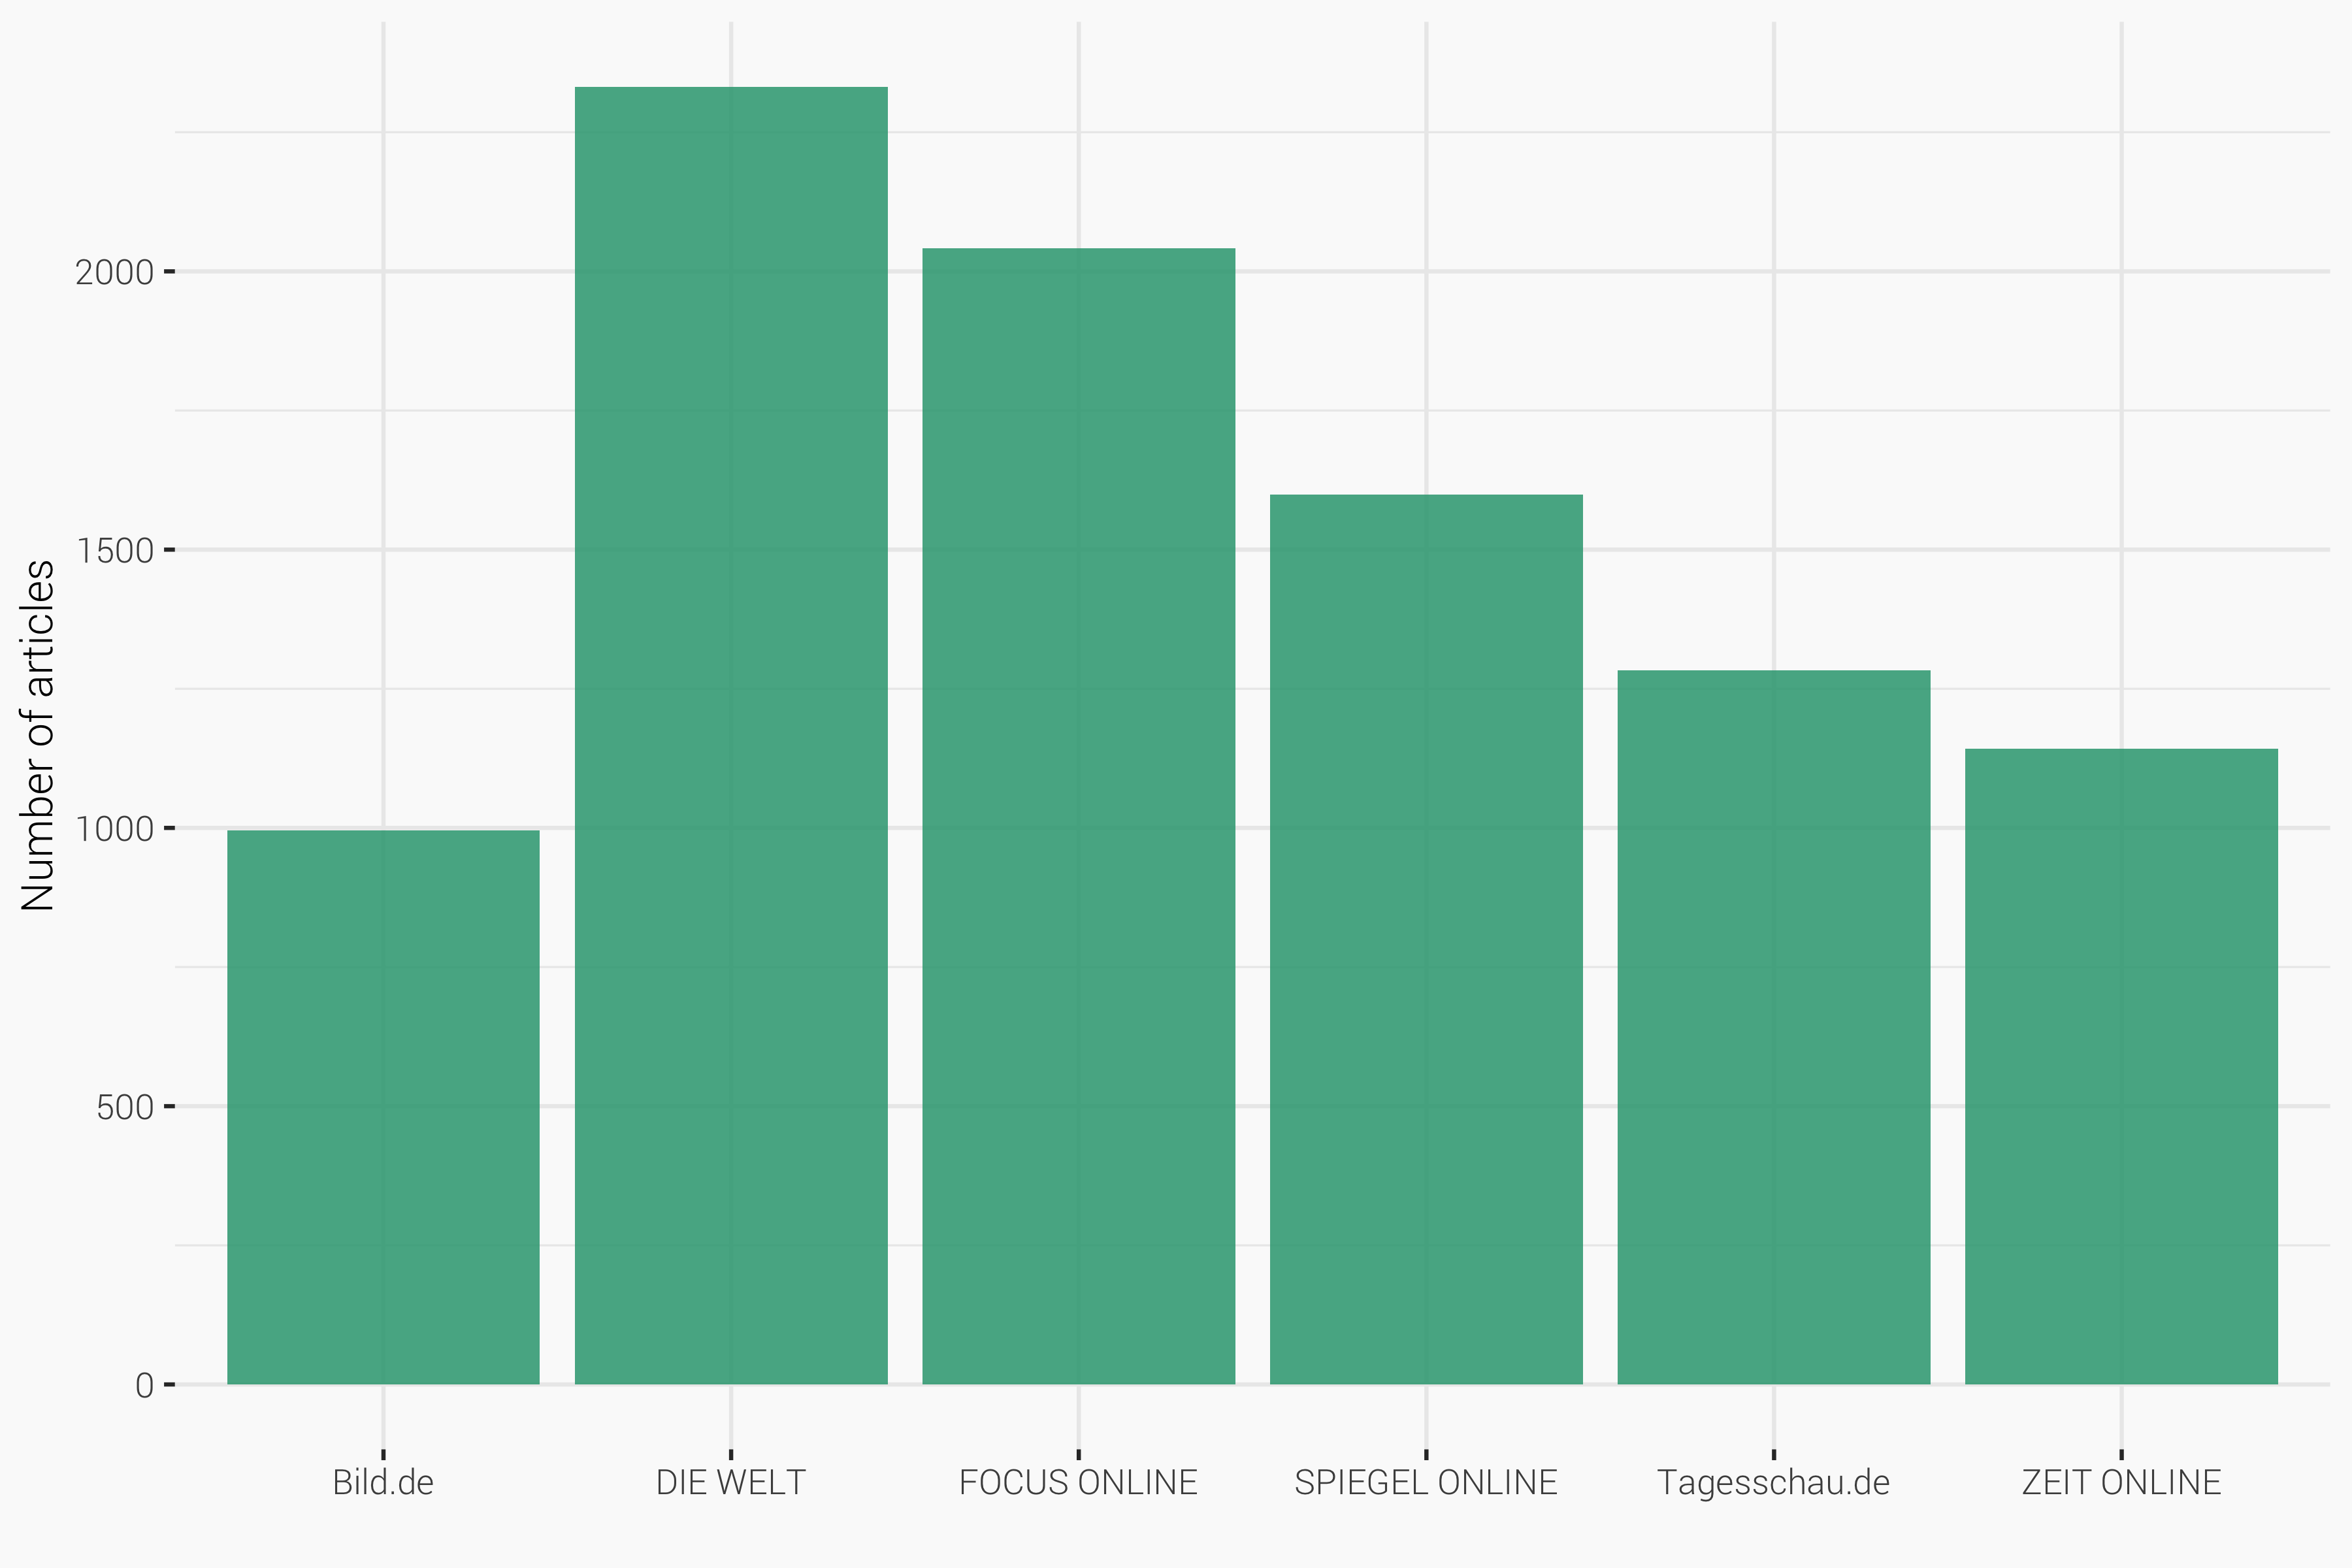
\includegraphics[width=\textwidth]{../figs/bar.png}
			\caption{... by news source}
		\end{subfigure}
	\end{center}
	\label{fig_distr}
\end{figure}

\begin{figure}[H]
	\caption{Distribution of Facebook shares...}
	\begin{center}
		\begin{subfigure}[normla]{0.49\textwidth}
			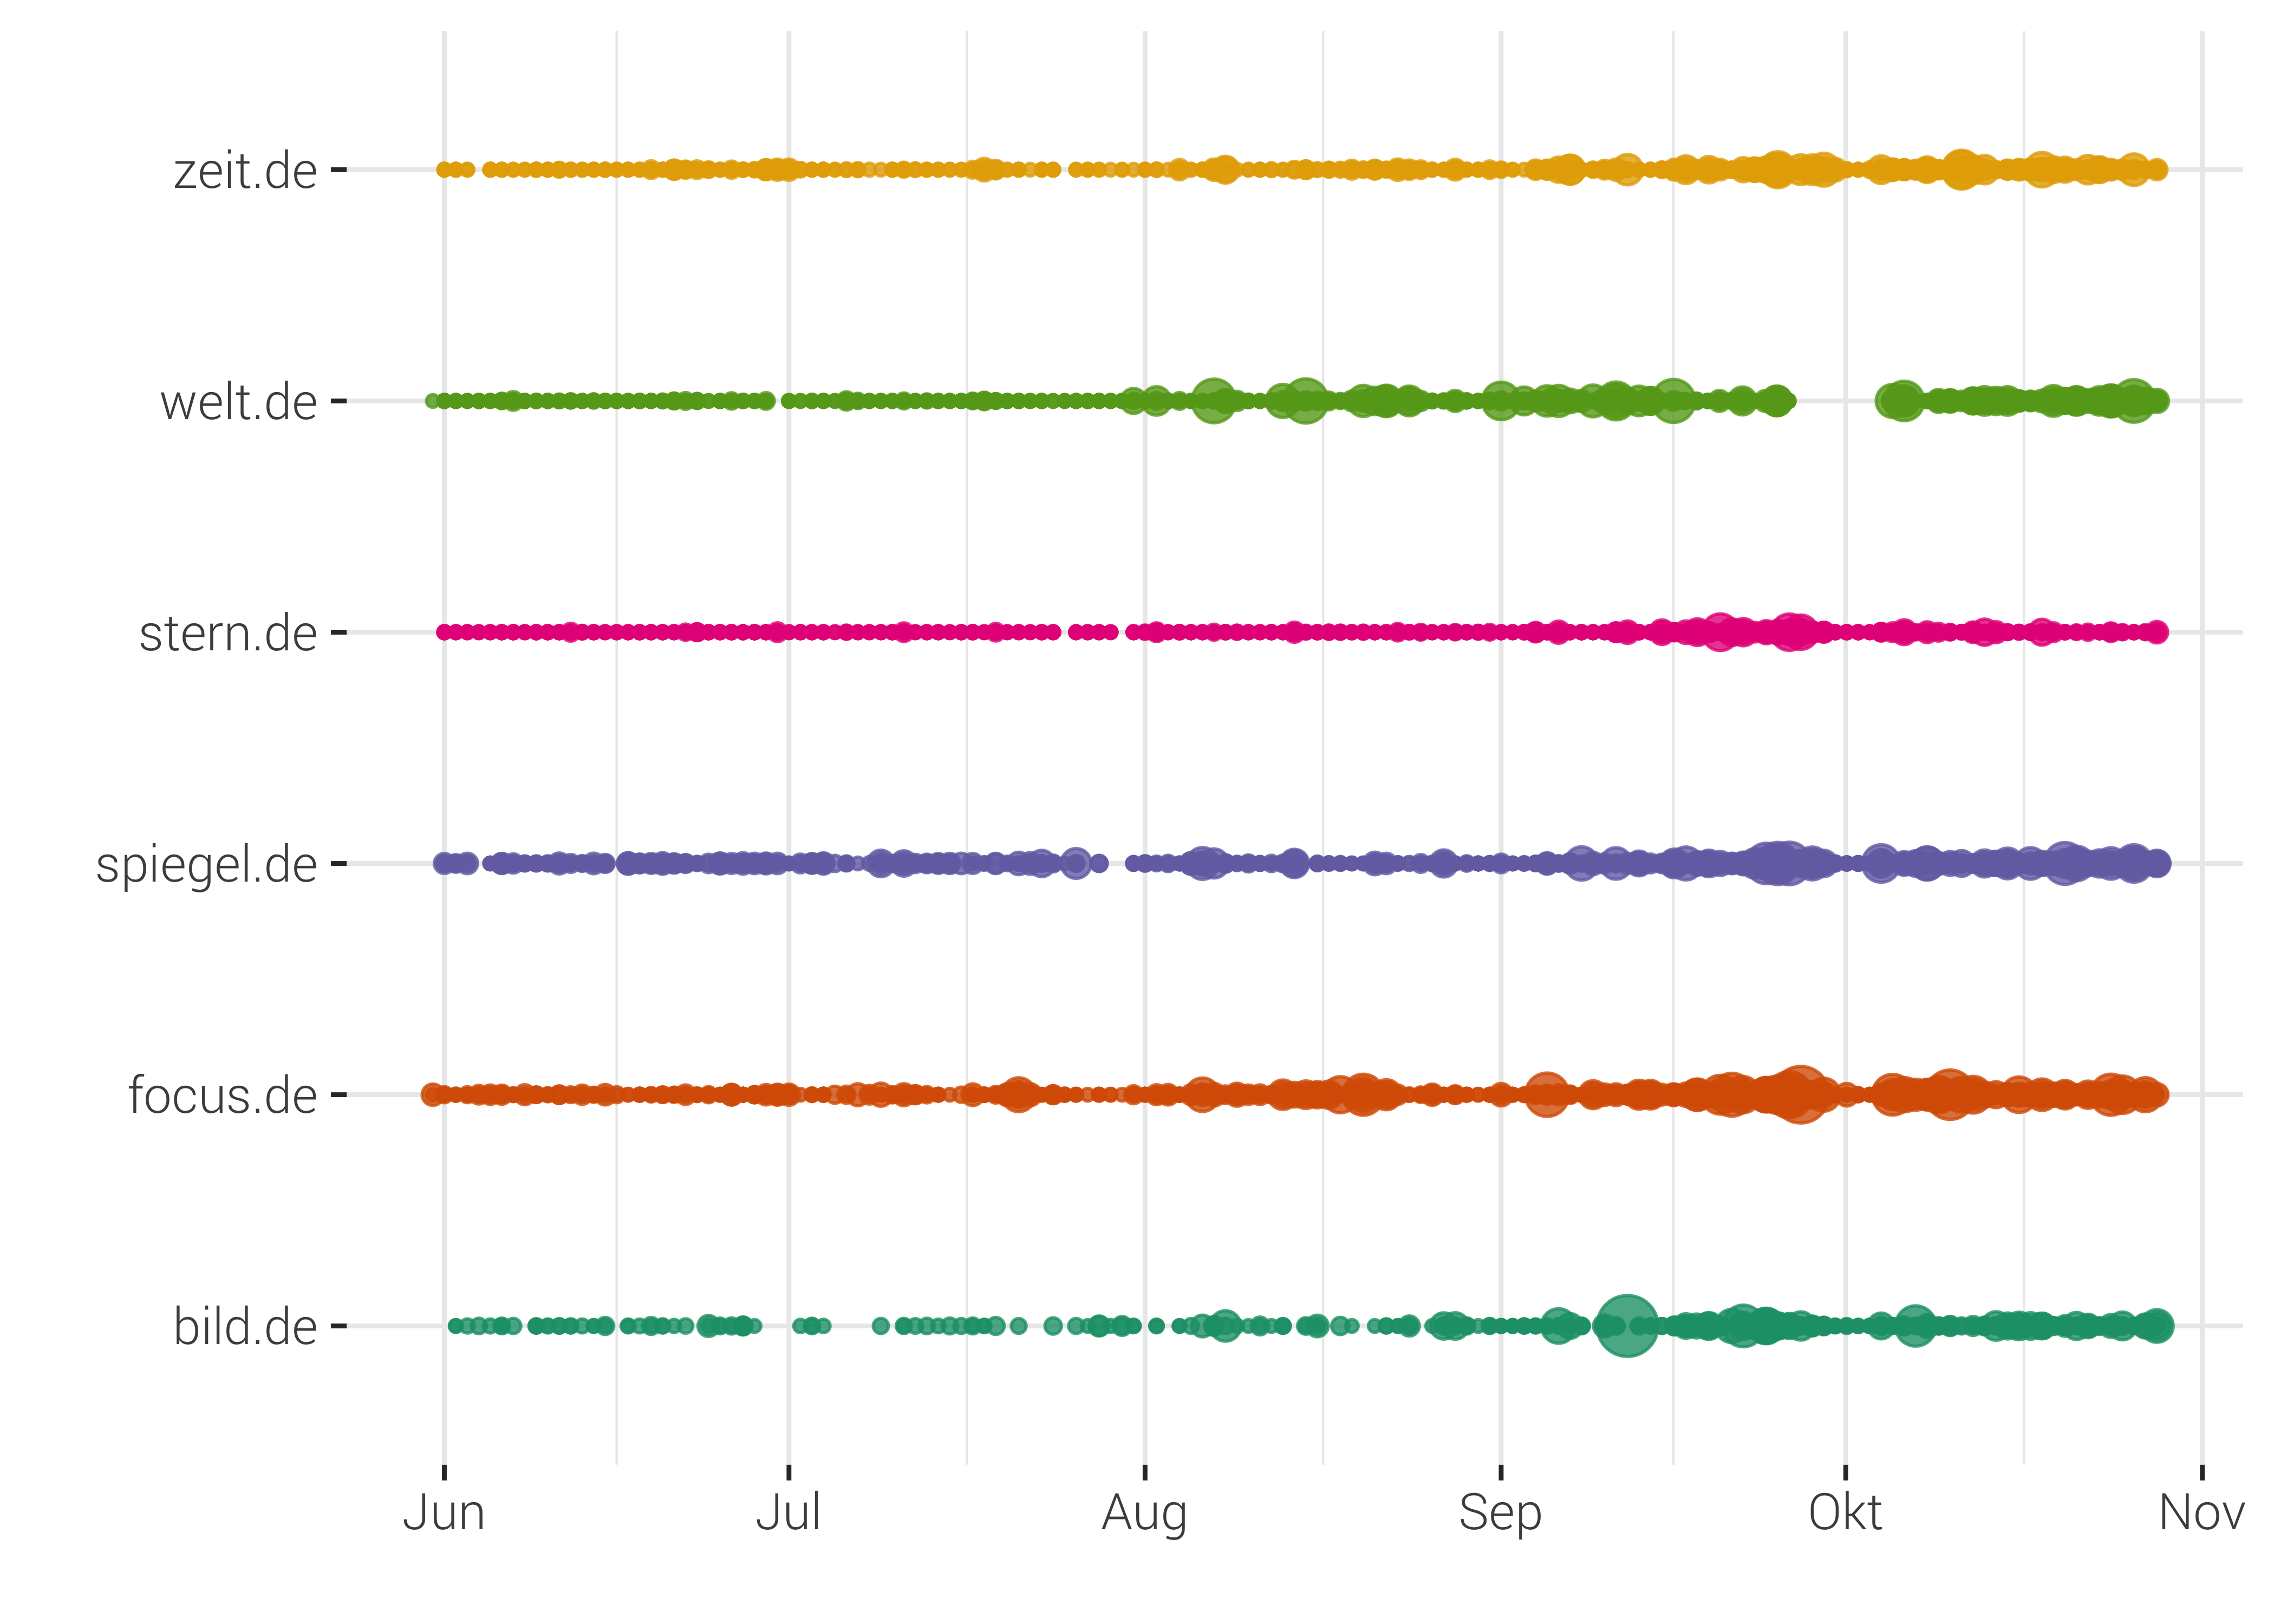
\includegraphics[width=\textwidth]{../figs/fb_shares.png}
			\caption{...by date \& news source}
		\end{subfigure}
		\begin{subfigure}[normla]{0.49\textwidth}
			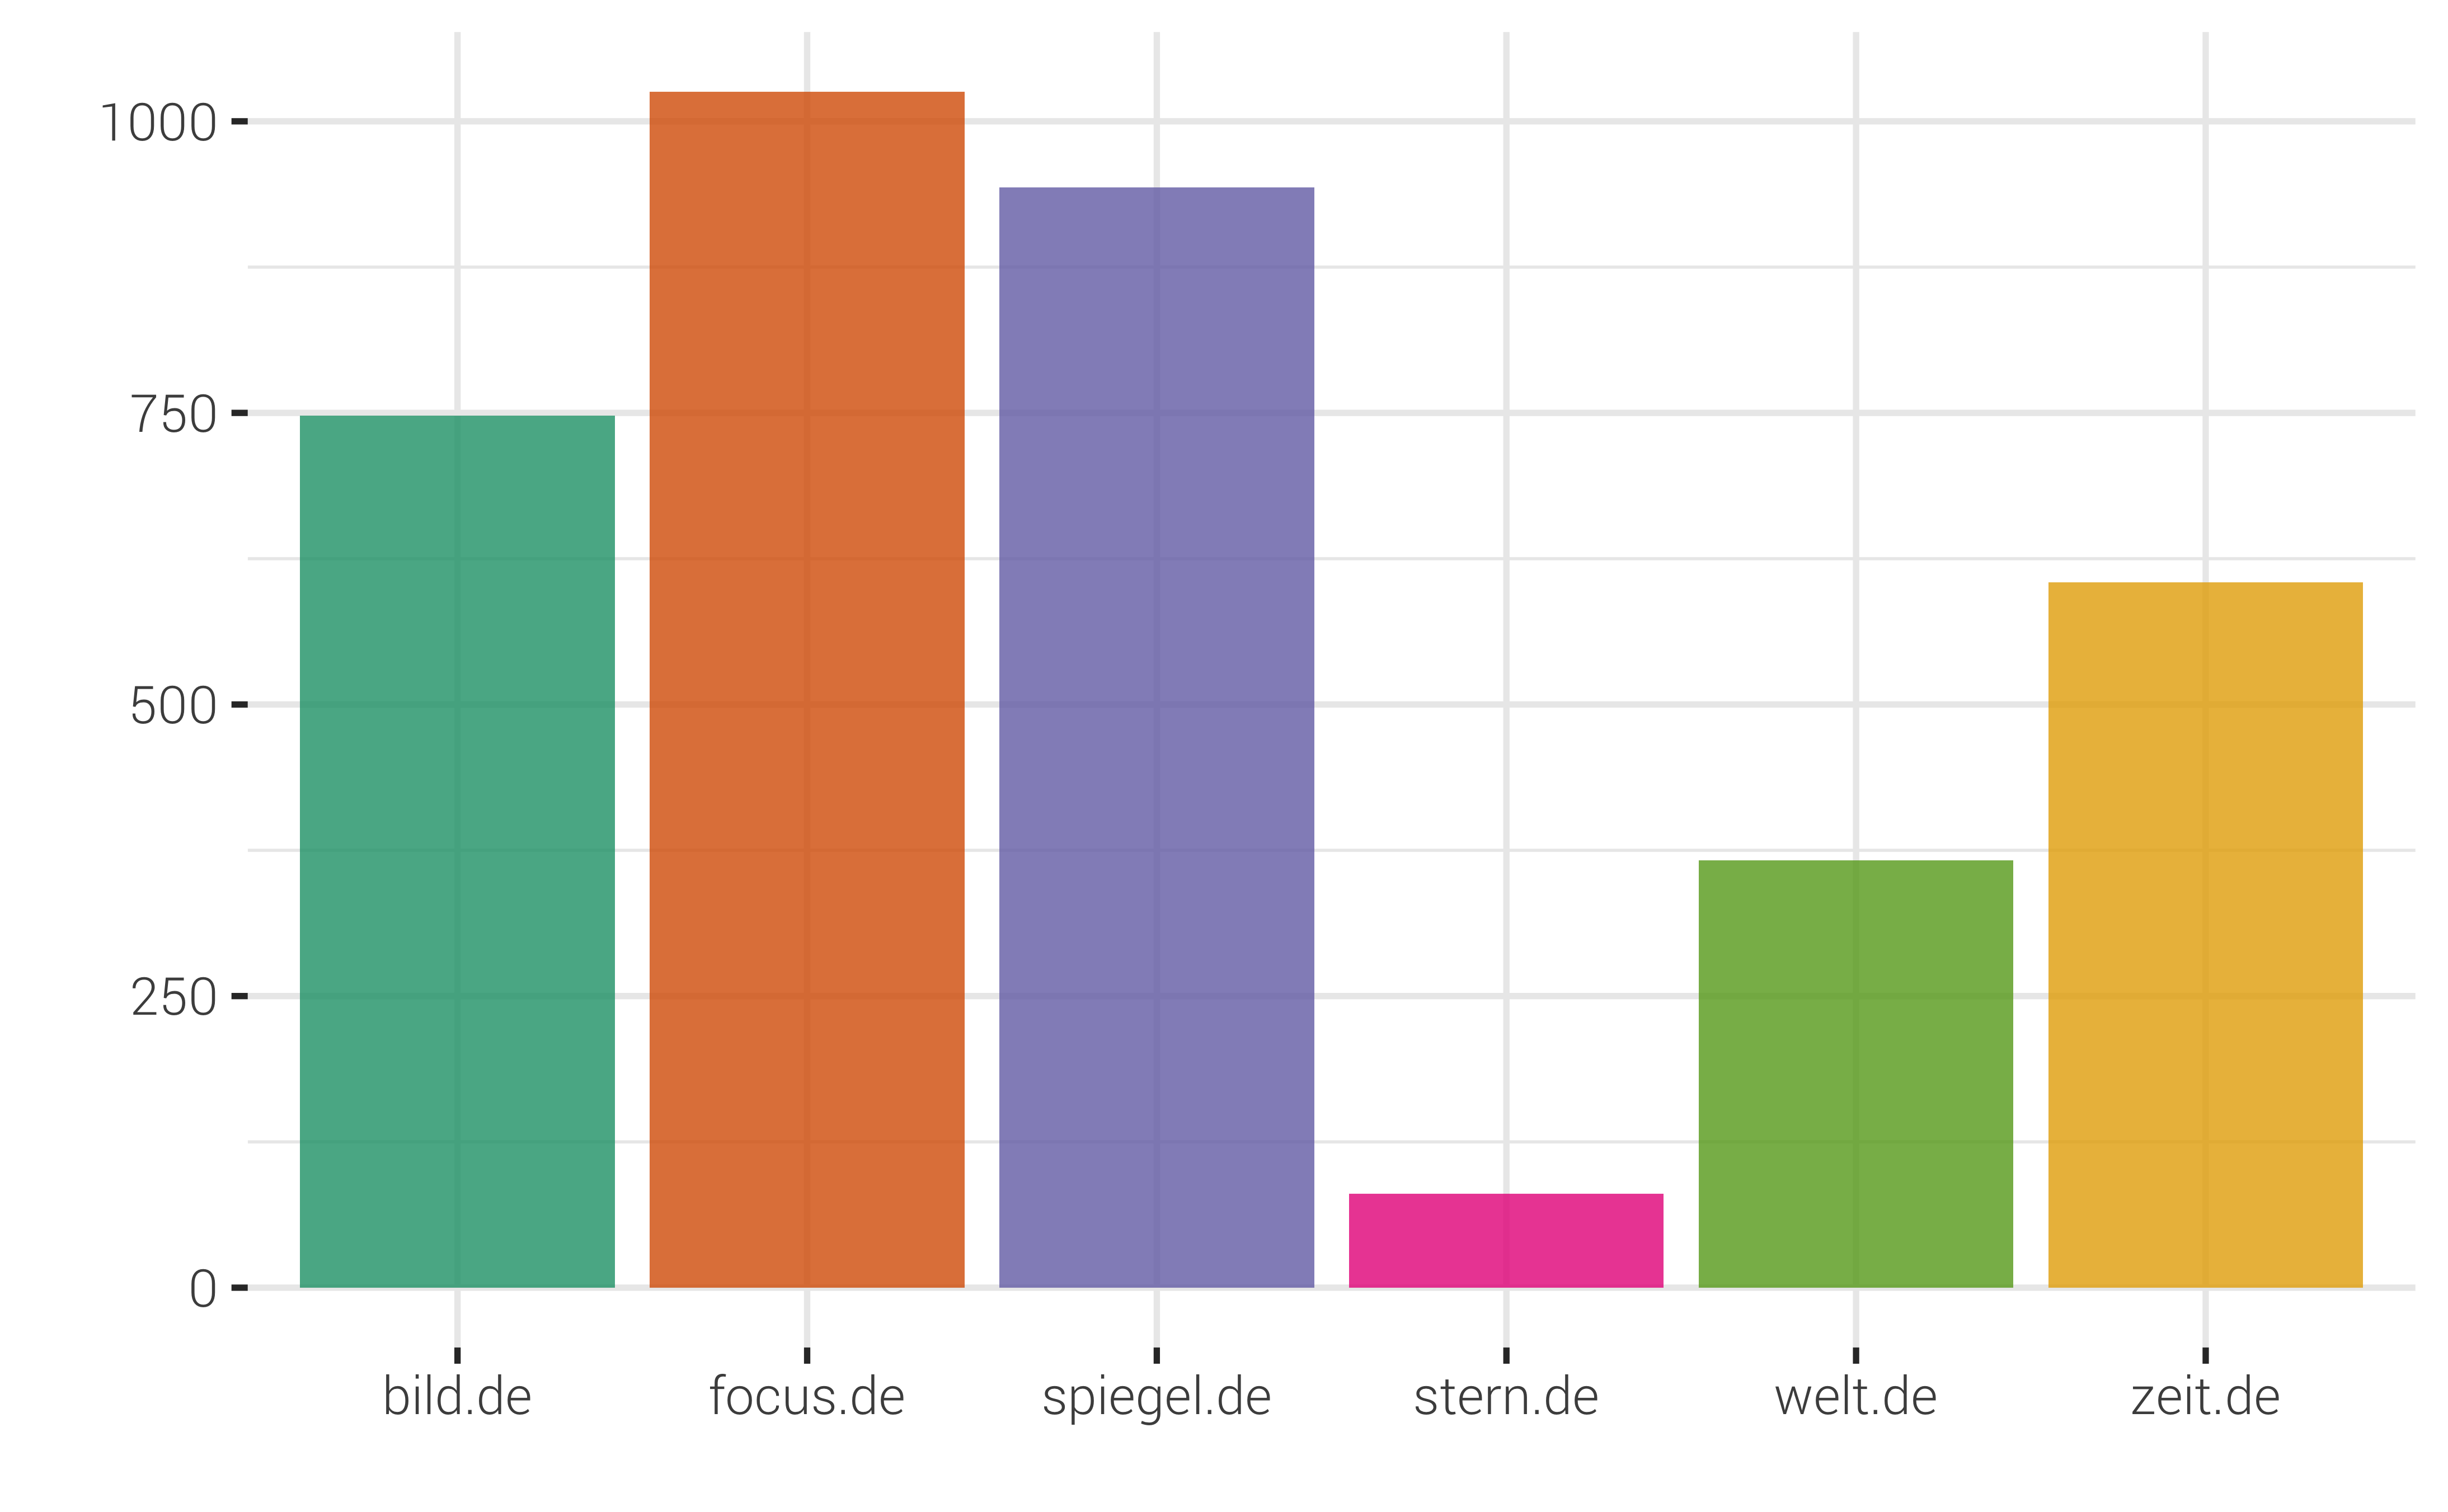
\includegraphics[width=\textwidth]{../figs/fb_shares_mean.png}
			\caption{... by news source (mean)}
		\end{subfigure}
	\end{center}
	\label{fig_fb_shares}
\end{figure}

To use text as data and reduce the dimensionality, a common strategy is to (a) pre-process the text by imposing some preliminary restrictions (stop-word removal, tokenization) based on the nature of the data (twitter text, newspaper articles, speeches, etc.) to reduce the number of language elements to consider and (b) limit the extent to which the dependence among elements within a document is encoded \citep{gentzkow_text_2017}. A raw text can than be represented as a term-document matrix, wehere each row is a numerical vector with each element indicating the frequency of a particular term in a document. In our case, a document is equivalent to a news article (title and body) and the collection of these documents are aggregated within a corpus. Any one document will contain only a subset of all unique terms, and the rows corresponding to unused terms will all be zero. 

% ------------------
% Text Pre-Procesing
% ------------------
\subsection{Text pre-procesing and feature selection}

A central task in text mining is to extract low-dimensional information from documents that are high-dimensional by nature \citep{bholat_text_2015}. This is related to the task of reducing the number of unique language elements in order to reduce the dimensionality of data (to avoid unnecessary computational complexity and overfitting) while at the same time keeping those words that reflect the content of a document. Any useful representation of text will throw away some information, as that is the essential purpose of text mining. The trick is to include the relevant information for our needs, and exclude the extraneous information. 

Intuitively the term frequency (tf) of a word is a measure of how important that word may be. There are words in a document, however, that occur many times but may not be important like articles, conjunctions, and so on. These terms, often called "stop words", are important to the grammatical structure of a text, but typically don't add any additional meaning and can therefore be neglected. We use a pre-defined stop word list from the Snowball stemmer project\footnote{http://svn.tartarus.org/snowball/trunk/website/algorithms/*/stop.txt} together with a customized stop-word list. We also remove punctuation character (e.g. ., ,, !, ?, etc.) and all numbers from our corpus.  

After pre-processing, each document (article) is a finite list of unique terms. Each unique term in the corpus is indexed by some $v \in \lbrace 1,...,V \rbrace$ where $V$ is the number of unique terms. For each document $d \in \lbrace 1,...,D \rbrace$ we compute the number of occurrences of term $v$ in document $d$ to obtain the count $x_{d,v}$. The $D$ x $V$ matrix $\boldsymbol{X}$ of all such counts is called the document-term matrix. This representation is often referred to as the bag of words model, since the order in which words are used within a document is completely disregarded. 

% ----------------------
% Structural topic Model
% ----------------------

\section{Topic detection}\label{ch_model}

As we do not observe the topics, we need to implement an unsupervised machine learning algorithm, that takes unclassified observations of words and uncovers hidden patterns (topics) that structure them in some meaningful way. We can than use the output of this process as inputs into an econometric model that predicts the number of Facebook shares \citep{gentzkow_text_2017}. 

We use the structural topic model (STM) developed by \citet{roberts_model_2016} that allows us to incorporate document specific covariates (e.g. author or date). STM is a recent extension of the standard topic modeling technique, the Latent Dirichlet Allocation (LDA). Topic models formalize the idea that documents are formed by hidden variables (topics) that generate correlations among observed terms. LDA is a particularly popular method for fitting a topic model \citep{blei_latent_2003}, also known as the generative aspect model \citep{minka_expectation-propagation_2002}. It treats each document $d$, containing $N_d$ words from a vocabulary of interest of $V$ unique terms, as a mixture of $k$ topics. Thus, each document has its own probability distribution over topics. Simultaneously, each topic is associated with a $V$-dimensional probability mass function $\boldsymbol{\beta}_k$, that controls the frequency according to which terms are generated from that topic. This standard topic modeling technique makes the assumption that all texts in the modeled corpus are generated by the same underlying process \citep{mishler_using_2015}. To include additional information that improve the estimation of the topics, we estimate a structural topic model, where topical prevalence (the distribution of topics among documents) is specified as a simple generalized linear model on document-level metadata. 

We use source of each article (the news-platform) as a covariate in the topic prevalence portion of the model with the data described above. Each document is modeled as a mixture of multiple topics. Topical prevalence captures how much each topic contributes to a document. Because different documents come from different sources, it is natural then to want to allow this prevalence to vary with metadata that we have about document sources. The observed words $w_i$ in a document are then viewed as the realization of some stochastic process.\footnote{See \citet{roberts_model_2016} for a formal description of the generative process.} We set the number of topics to be 40 after evaluating and maximizing topics' coherence using a cross-validation scheme while changing the number of topics (\citet{airoldi_reconceptualizing_2010}; \citet{roberts_model_2016}).

\section{Probabilities and Classification}\label{ch_results}


After performing the topic modeling, we can generate an overview of the news landscape about the german elections. Each group is composed of the most relevant words for that topic, and a manually-determined label. The distances that the topics have from each other reflect their semantic distance, or basically how different the words are for that topic. It is computed as the Jensen-Shannon divergence between each of the topics according to the differences in their word-topic probabilities. We then apply principal coordinates analysis in order to project the distance matrix down to two dimensions.

\begin{figure}[H]
\centering
	\caption{News Landscape}
	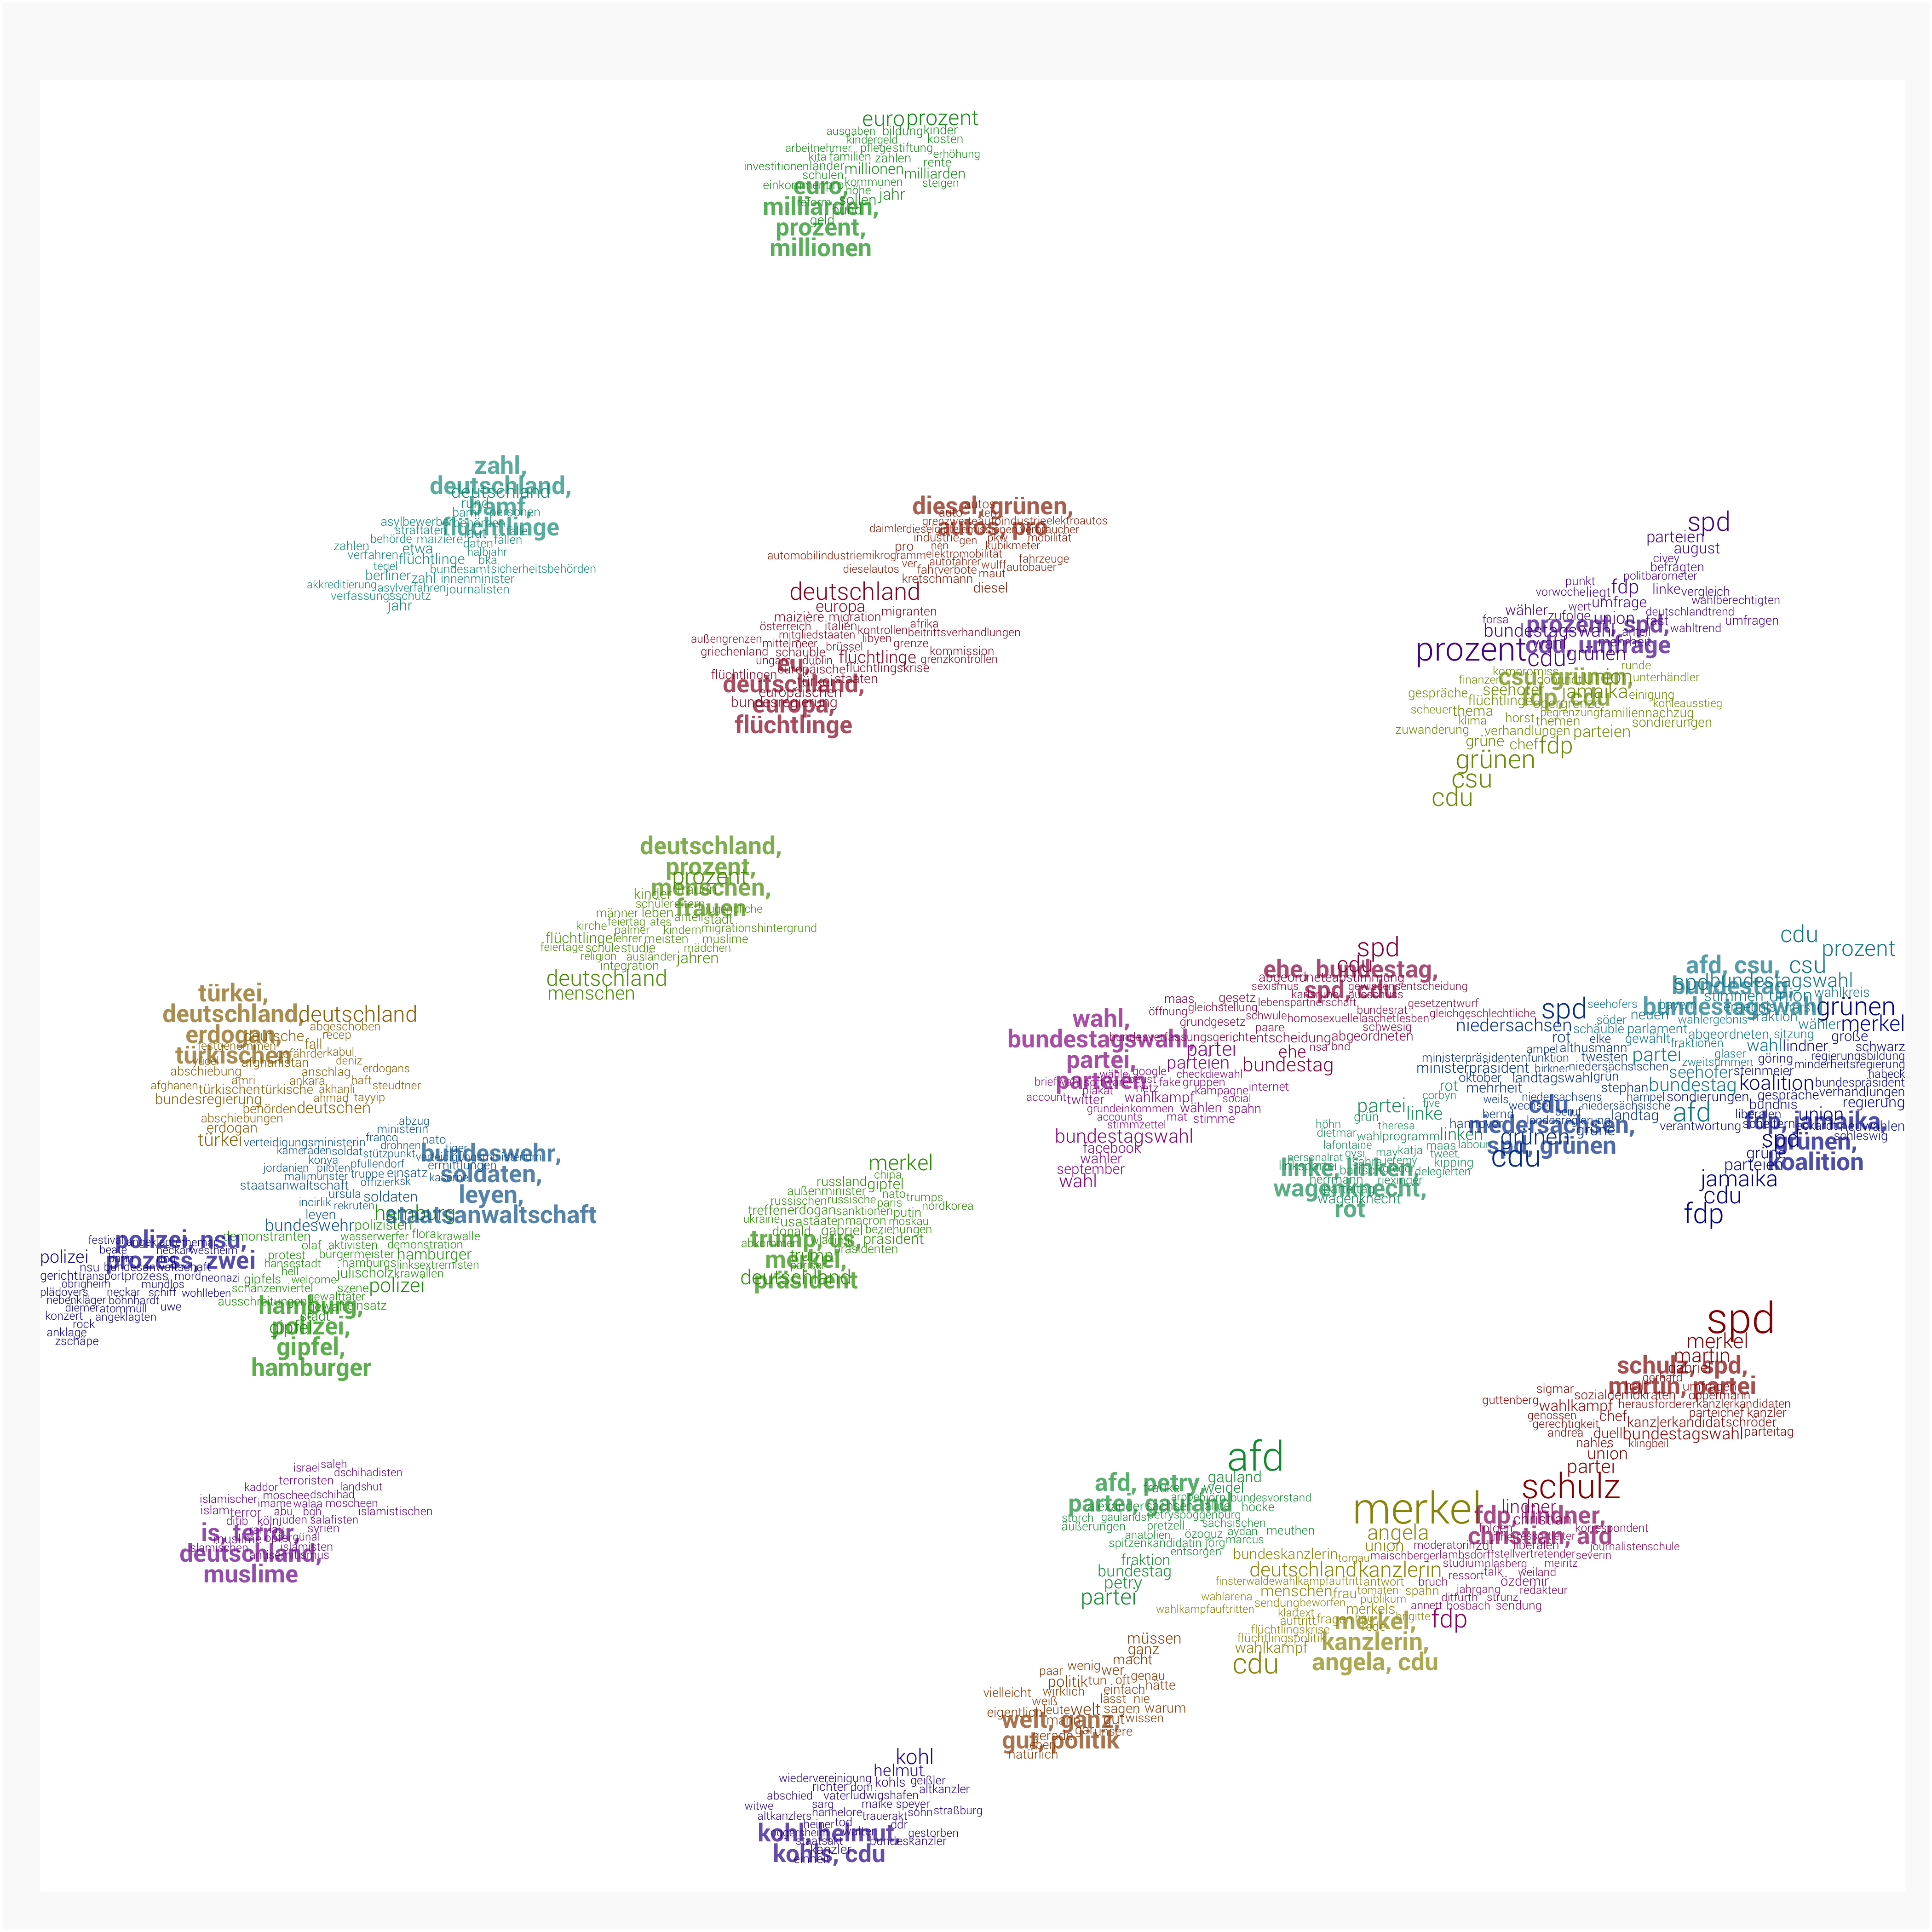
\includegraphics[width=\textwidth]{../figs/news-landscape-map.png}	
	\label{fig_landscape}
\end{figure}

To check weather the estimated topic classifications make sense, we first produce sample documents classified to that topic for reference. We produce a random sample of 10 posts from the 300 highest probability fits per topic.

\begin{figure}[H]
\centering
	\caption{Sample articles}
	\includegraphics[width=\textwidth]{../figs/topic-classification-sample.png}	
	\label{fig_classification}
\end{figure}

\begin{figure}[H]
\centering
	\caption{Sum of Facebook shares by topic}
	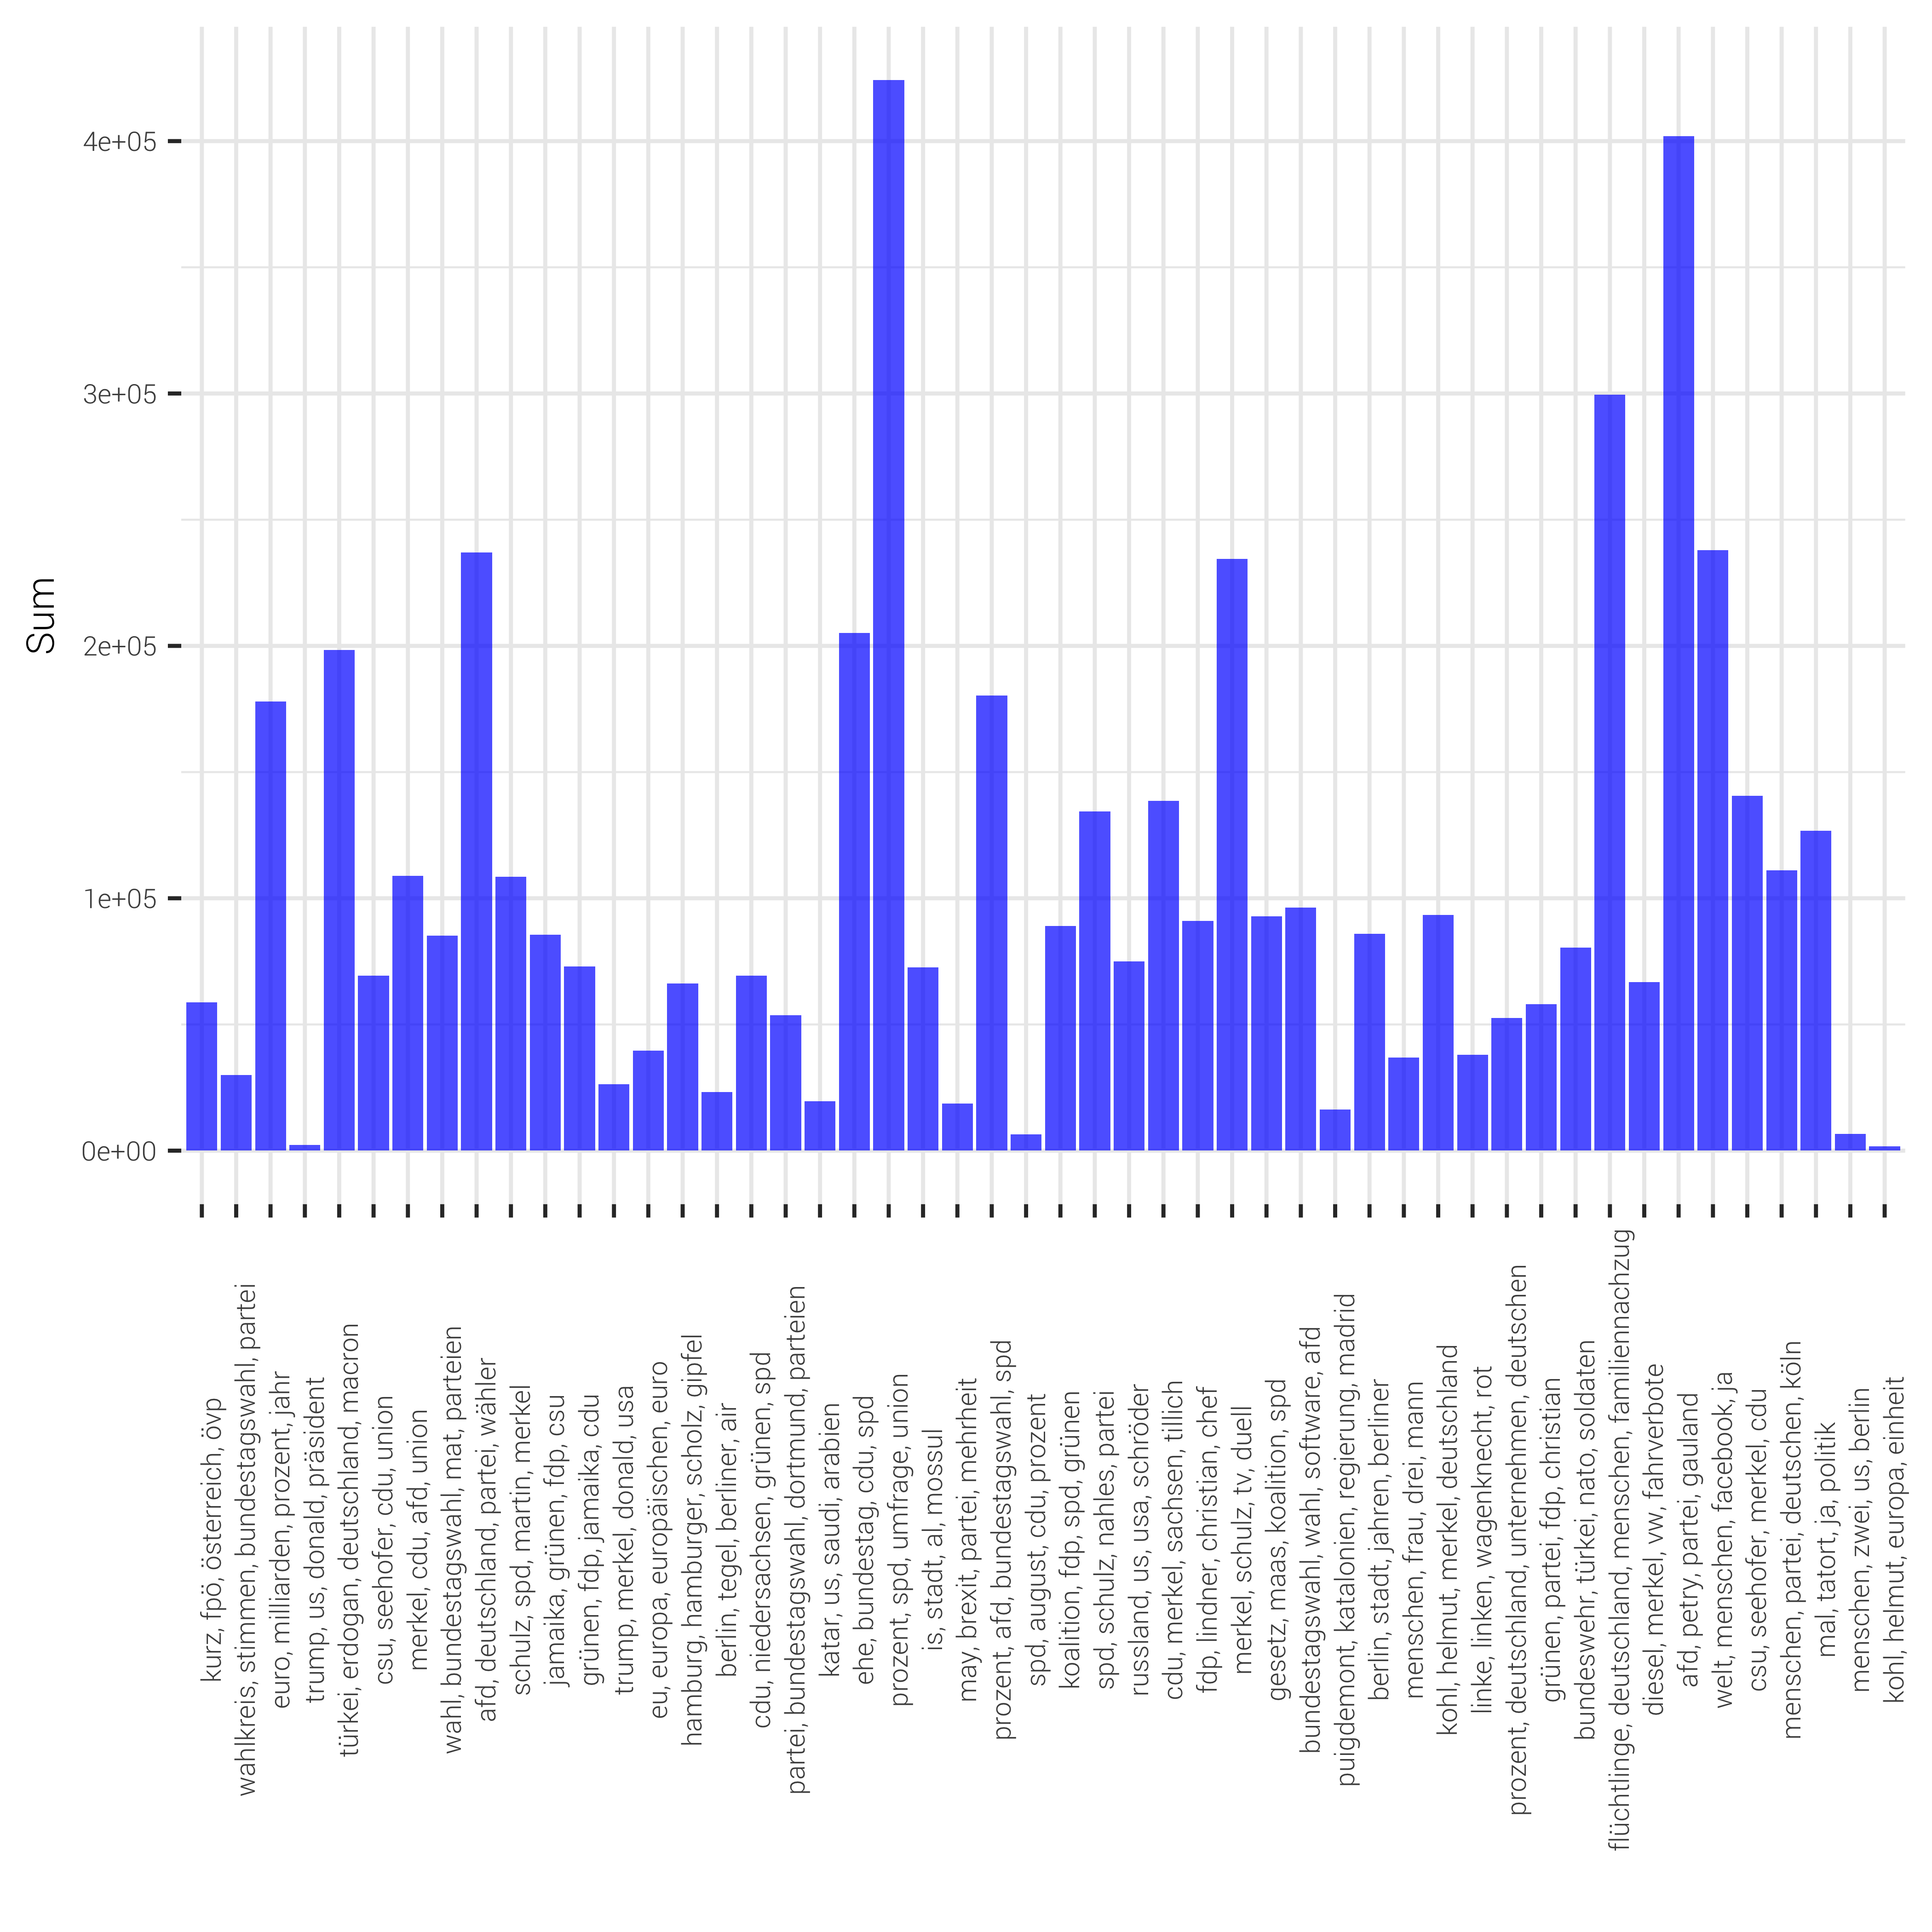
\includegraphics[width=\textwidth]{../figs/fb_shares_topics.png}	
	\label{fig_fb_shares_topic}
\end{figure}

\section{Regression}\label{ch_regression}

\end{document}
